\documentclass{article}


% if you need to pass options to natbib, use, e.g.:
%     \PassOptionsToPackage{numbers, compress}{natbib}
% before loading neurips_2024


% ready for submission
\usepackage{neurips_2024}


% to compile a preprint version, e.g., for submission to arXiv, add add the
% [preprint] option:
%     \usepackage[preprint]{neurips_2024}


% to compile a camera-ready version, add the [final] option, e.g.:
%     \usepackage[final]{neurips_2024}


% to avoid loading the natbib package, add option nonatbib:
%    \usepackage[nonatbib]{neurips_2024}

\usepackage{graphicx} 
\usepackage[utf8]{inputenc} % allow utf-8 input
\usepackage[T1]{fontenc}    % use 8-bit T1 fonts
\usepackage{hyperref}       % hyperlinks
\usepackage{url}            % simple URL typesetting
\usepackage{booktabs}       % professional-quality tables
\usepackage{amsfonts}       % blackboard math symbols
\usepackage{nicefrac}       % compact symbols for 1/2, etc.
\usepackage{microtype}      % microtypography
\usepackage{xcolor}         % colors

\usepackage{biblatex} %Imports biblatex package
\addbibresource{bibliography.bib} %Import the bibliography file

\title{Semiconductor Layout Design with Large Language Models: Opportunities and Challenges}

\author{%
  Bo Wen\\
  IBM Watson Research Center, \\
  Yorktown Heights, NY, USA \\
  \texttt{bwen@us.ibm.com} \\
  \And
  Xin Zhang\\
  IBM Watson Research Center, \\
  Yorktown Heights, NY, USA \\
  \texttt{xzhang@us.ibm.com} \\
}

\begin{document}

\maketitle

\begin{abstract}
  % Update abstract to reflect the content of the paper
  This paper explores the potential of large language models (LLMs) as a ``layout design copilot'' in various domains such as semiconductor, IC, and microfluidics. We evaluate the capabilities of LLMs in generating basic elements and combining them into complex designs. Our experiments focus on via connections, microfluidics channel design, and fiducial marker generation. We discuss the opportunities and challenges of using LLMs in layout design, highlighting the importance of providing expert knowledge and context to improve their performance.
\end{abstract}

\section{Introduction}
The semiconductor industry faces significant challenges in automating the layout design for integrated circuits (ICs), microfluidic chips, and other electronic devices. Current graphical user interface (GUI) based design workflows lack adaptability, leading to inefficient, repetitive tasks when creating similar structures with minor variations.\cite{Greengard2024-hx} This approach violates the ``Don't Repeat Yourself'' (DRY) principle and reduces productivity.

While traditional layout design software has struggled to address these challenges, Large Language Models (LLMs) offer a promising solution. LLMs' ability to understand natural language instructions and generate code makes them ideal candidates for a ``layout design copilot''. This new paradigm could allow human designers to focus on high-level tasks requiring creativity and intuition, while the LLM-powered copilot generates or modifies the layout code based on human intent.

In this paper, we explore the capabilities and limitations of LLMs with 25 common semiconductor layout design tasks. Our main contributions are: 
(1) Evaluating the baseline performance of five state-of-the-art LLMs on layout design tasks with zero-shot prompting; Identifying common errors and proposing how to use Retrieval-Augmented Generation (RAG) and In-Context Learning to address them (Section 2). 
(2) Documenting an iterative design process of multimodal inputs with GPT-4o for a complex task (ViaConnection), illustrating the limitations of current LLMs in spatial reasoning (Section 3). 
(3) Introducing a novel Neuro-inspired LLM Reasoning Network architecture that leverages multiple LLMs to improve reasoning capabilities and mitigate hallucinations in layout design tasks. Presenting preliminary results. (Section 4).

Finally, Section 5 concludes the paper and discusses future research directions.

\section{Baseline LLM Performance in Layout Design}

We evaluated the performance of five large language models (LLMs) - GPT-4o\cite{GPT-4o}, Claude-3.5-Sonnet\cite{Claude-3.5-Sonnet}, Llama-3.1-70B\cite{Llama-3.1-70B}, Llama-3.1-405B\cite{Llama-3.1-405B} and the new ``reasoning model'', o1-preview\cite{o1-preview} - on a set of 25 layout design tasks. Each tasks have been run 5 times with same prompt and temperature = 0.7. The LLMs are asked to write a python code with gdspy\cite{gdspy} and generate a GDSII file. We then run the LLM written code in a Linux VM and further convert the generated GDSII file to png images for human evaluation. These tasks were categorized into four groups: Basic Shapes 1, Basic Shapes 2, Advanced Shapes, and Complex Structures. Figure \ref{fig:baseline-llm-performance} presents a summary of the LLMs' performance across the task categories. See Appendix for the task prompts and detailed results.

\begin{figure}[h]
  \centering
  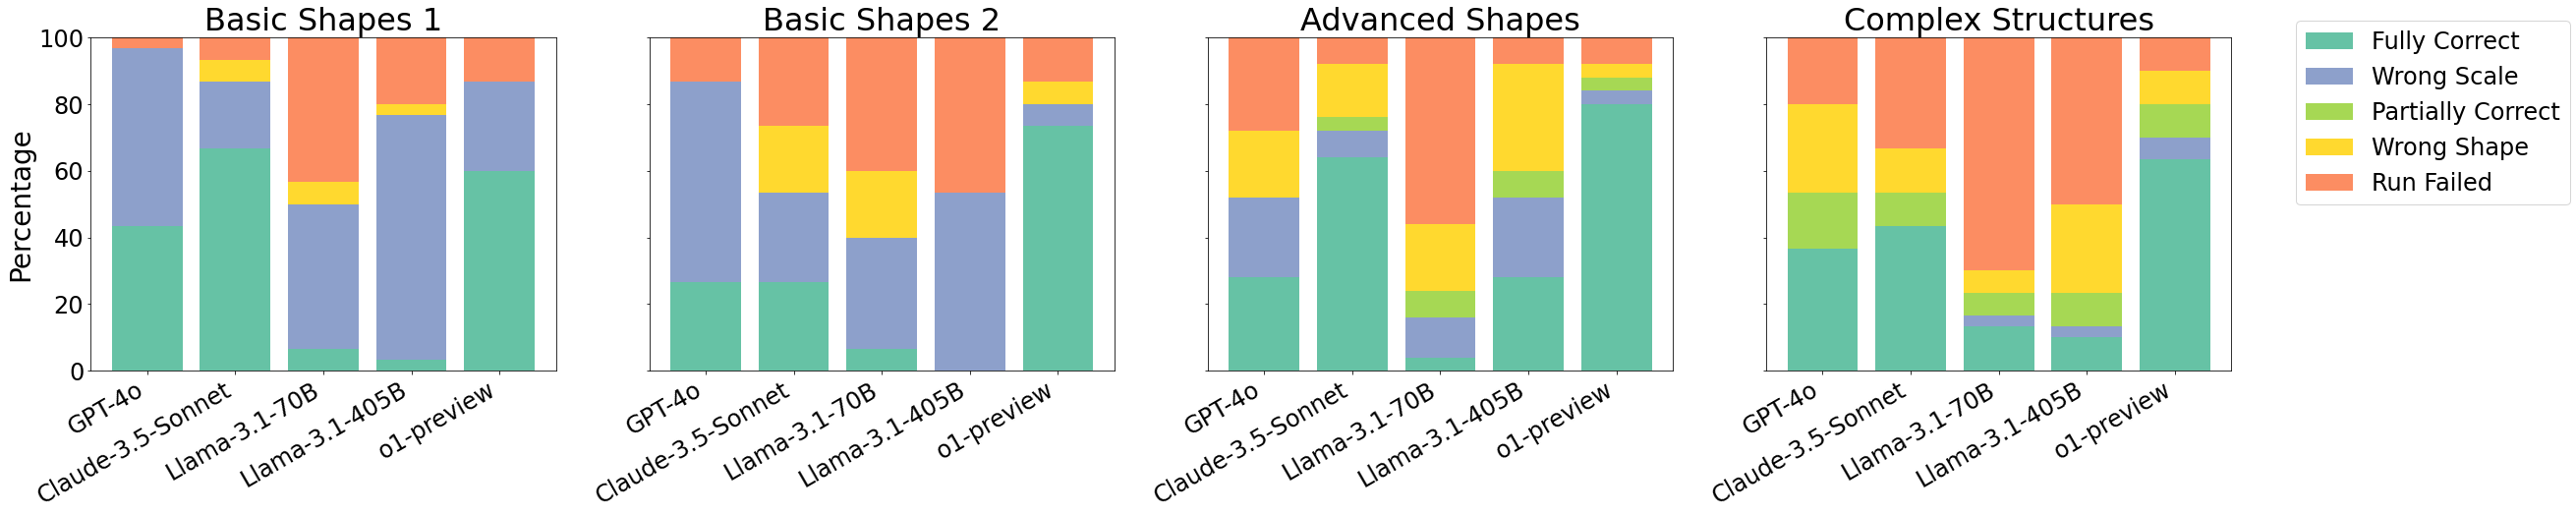
\includegraphics[width=\textwidth]{baseline-llm-performance.png}
  \caption{Baseline LLM Performance on Layout Design Tasks}
  \label{fig:baseline-llm-performance}
\end{figure}

The results reveal several common mistakes and limitations of standalone LLMs in handling layout design tasks:

  1. \textbf{Incorrect scaling}: The default unit in the gdspy library is micrometers. But we requested the basic shapes to be drawn in millimeters, in order to test whether the LLM could correctly figure out this catch and scale the shapes according to the specified units. As can be seen from the dark blue ``Wrong Scale'' part of bar chart, all the LLMs struggled to various degrees: (a) Sometimes the LLMs simply failed to pay attention to the requested unit (millimeters) and did not perform the necessary scaling. (b) In some cases, LLMs did pay attention to the requested unit but made incorrect assumptions about gdspy's default unit. We observed many hallucinations of millimeters and resulting in no scaling. Interestingly, we observed one case where Claude-3.5-Sonnet hallucinated that the default unit was nanometers, leading it to scale the length by 1e6. This resulted in shapes too large to be drawn. (c) From the chart, we can see that Llama-3 models are especially vulnerable to this issue. They sometimes even assumed the user had made a mistake by requesting millimeters, and proceeded to draw in micrometers instead, justifying this choice with comments like "not mm, as the GDSII format is in micrometers". This type of ``arrogant'' behavior and misalignment with human instructions on simple tasks will be very harmful for deploying LLMs as fully automanous AI agents. A recent Nature paper \cite{ZhouNature2024} has also discussed similar observations.
  
  2. \textbf{Partial correctness}: In more complex tasks, LLMs often generated partially correct layouts with mistakes in the relative positioning of simple shapes. For example, in the ViaConnection task, which involved specific relative location requirements like ``Ensure the metal connection fully covers the vias and leaves a margin of 10 units between the edge of the metal and the pads. Leave a space of 50 units between the vias and the edges of the metal connection.'', only o1-preview achieved one fully correct result. The other LLMs all produced partially correct outputs as shown in the yellow ``Partially Correct'' part of the bar chart.
  
  3. \textbf{Runtime errors}: Approximately one third of the generated code from the evaluated LLMs resulted in exceptions and failed to execute. The most frequent error, \textit{AttributeError: module 'gdspy' has no attribute 'LayoutViewer'}, occurred 26 times (59.09\%) with GPT-4o and 33 times (61.11\%) with Claude-3.5-Sonnet. In contrast, this error was reported only once each for Llama-3.1-70B and o1-preview, and not at all for Llama-3.1-405B, indicating that GPT-4o and Claude-3.5-Sonnet are trying to be more ``helpful'' by providing GUI output, which is not available in the runtime environment. This is not entirely LLM's fault, but due to missing information in the prompt. The second most common errors were due to hallucinations of nonexistent `gdspy` functions or methods, including various `AttributeErrors` (e.g., `'CrossSection'`, `'Circular'`, `'Ellipse'`) and `TypeErrors`. This also includes spelling error, for example, miss spelling \textit{gdspy.Text} as \textit{gdspy.text}. Additionally, other frequent issues involved typical programming logic mistakes such as missing module imports or incorrect function parameters. For more details, see the error report in (Appendix).
  
  4. \textbf{Inefficient code}: There's one special case that we'd like to point out. In the DLDChip task, which involves creating a dense array of identical shapes, the Llama-3.1-405B model generated a code that created a large number of objects and performed numerous boolean operations, leading to high memory usage and extended execution time. We have to kill the code after about 15 mins of waiting. 

  5. \textbf{Ambiguous instructions}: In some of the results, we observed that the LLMs results mainly fall into two categories. After inspecting the prompts, we found that the instructions can be interpreted in two ways. In this case, we count both type of results as correct. But when implementing copilot, the agent should ask for clarification if the instructions are ambiguous.

Many of these issues can be mitigated by augmenting the LLMs with more advanced setup. For example, using Retrieval-Augmented Generation (RAG) to provide gdspy documentation to the LLMs, we should be able to reduce the errors related to misspelling and hallucinating nonexistent functions. For complex tasks, we can provide example code of simple shapes for In-Context Learning, so the LLMs only need to reason about positioning and scaling, and avoid runtime errors. We will discuss more in Section 3.

\section{Multimodal Inputs and Spatial Reasoning}
Layout design in semiconductor processes requires not only generating correct basic geometric shapes but also spatial reasoning to create proper ``layouts'' that meet specific requirements. Via connections, which create electrical pathways between different chip layers, exemplify this challenge. While seemingly simple—typically consisting of circular vias and rectangular metal connections—they demand precise positioning and sizing to ensure no short or open circuits and other functionality issues.

Our baseline experiments revealed that LLMs most frequently producing ``Partially Correct'' outputs in the ViaConnection task as expected. Llama-3.1-405B once, GPT-4o and Llama-3.1-70B twice, Claude-3.5-Sonnet and o1-preview 3 times. This observation motivated us to use ViaConnection as a testbed to further explore LLMs' spatial reasoning capabilities.

We conducted a series of tests by providing a sketch(image) together with text prompt to help LLM understand the spatial relationships. The sketch are color-coded to represent different layers (e.g., yellow for via, blue for metal, red for pad). The text prompt specified layer information, dimensions, positions, and connectivity requirements. We used GPT-4o's vision input capability for this experiment. Figure \ref{fig:via_experiment} illustrates the sketch inputs and corresponding LLM-generated outputs for each test case.

\begin{figure}[!h]
\centering
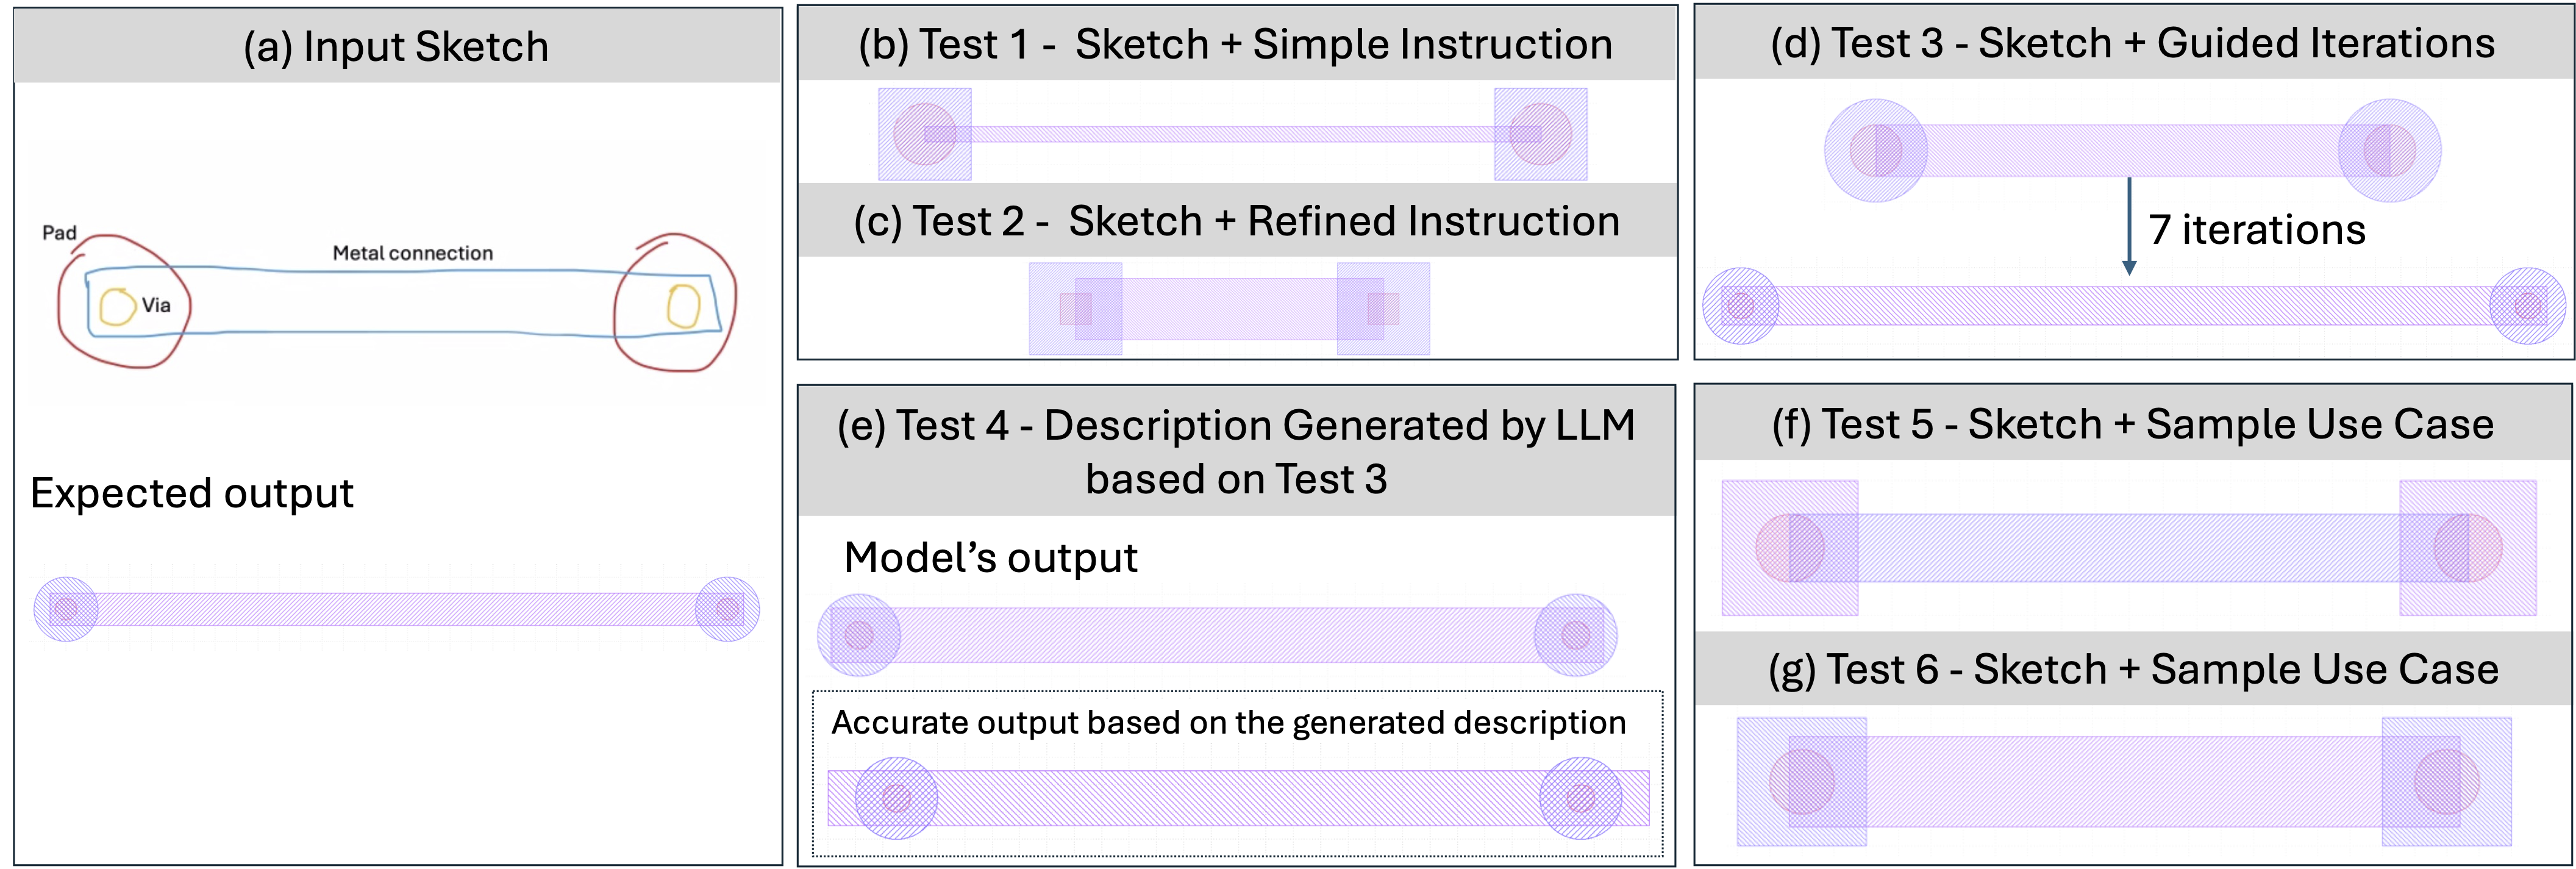
\includegraphics[width=1\linewidth]{Styles/Figure1_v5.png}
\caption{Sketch input and LLM-generated outputs for the via connection experiment. The sketch depicts a desired layout with two vias connected by a metal layer and circular pads on top. The outputs show the progression of the LLM's understanding and refinement of the layout based on iterative feedback and context provided by the user.}
\label{fig:via_experiment}
\end{figure}
In \textbf{Test 1}, we provided a basic sketch (Figure ~\ref{fig:via_experiment}(a)) along with a simple instructions (Appendix) to inform it each color represented a different layer. The LLM generated code based on this initial description; however, the output presented several issues, including the metal connection's width is insufficient to fully cover the vias. \textbf{Test 2} involved refining the description (Appendix), however the output has the vias in square instead of square, and the model also failed to have metal connection fully cover and extend slightly beyond the two vias. In addition, both cases misplaced the padding in square as supposed to be circle 

In \textbf{Test 3}, we provided a more detailed description (Appendix) accompanied by the original sketch. The initial output generated by the LLM did not fully cover the vias with the metal connection, and the metal width was narrower than the via's radius. To guide the model to generate code to draw the expected output, we proceeded with an iterative process, providing the LLM with feedback and screenshots of the GDSII file generated from its code. After seven iterations, the LLM successfully produced the correct layout (Appendix). \textbf{Test 4} aimed to reproduce the best output from the previous test. We requested the LLM to create a detailed prompt based on the successful result from Test 3 (Appendix) and used this prompt to attempt to generate the correct output again. However, the description didn't accurately describe the desired output. The generated description asked for \textit{a space of 50 units between the vias and the edges of the metal connection.} Based on this description, the accurate output should be like the one in dotted rectangle in Figure~\ref{fig:via_experiment}e, with the metal extends beyond the padding. Interestingly, when using this description to ask the model to generate code for the design, the output matches the one originally expected. 
% the description is not specific enough. non expert won't be able to tell the difference between the correct and wrong via connection in the image.

\textbf{Tests 5} and \textbf{6} gradually incorporated more context, such as 3D packaging, Through-Silicon Vias (TSVs), and other domain-specific requirements. However, adding domain knowledge and context did not improve the LLM's performance much, showcasing both its limitations and areas for potential improvement. Experienced engineers and researchers understand that connecting two vias requires using a metal layer wider than the diameter of the via and fully covers the vias. Moreover, vias should not be placed at the very ends of metal layers; some leeway is typically be left between layers to accommodate potential misalignment. % this last part is good. very specific.

Our experiments reveal a critical limitation in LLMs' ability to adapt to domain specific applications. Despite possessing general semiconductor knowledge, LLMs struggle to translate this understanding into accurate spatial relationships, as evident in Tests 5 and 6, where additional domain context did not improve results. Notably, the o1-preview model, with its enhanced reasoning capabilities, demonstrated better performance, suggesting that using domain knowledge to reason about geometric constraints is crucial for advancing their performance in layout design tasks. This finding also highlights that finetuning LLMs to improve reasoning and understanding how to apply domain knowledge in problem-solving is more important than increasing model size to remember more knowledge, which is key to improving the adaptability of LLM-based AI systems.

\section{Neuro-inspired LLM Reasoning Network Architecture}

In this section, we present a novel Neuro-inspired LLM Reasoning Network Architecture designed to enhance the reasoning capabilities of large language models (LLMs) and mitigate the issue of hallucinations in generated outputs. This architecture is particularly well-suited for complex domains such as semiconductor layout design, where the ability to generate accurate and consistent results is critical.

The proposed architecture is inspired by the Brain-like AGI and the Free Energy Principle (FEP) theory. It consists of three main components: Thought Generator Pool, Thought Assessors, and a Steering Subsystem. The Thought Generator Pool is a multi-LLM network that generates initial attempts at a given task by exploring different approaches and perspectives. This multi-LLM approach allows for a more comprehensive exploration of the problem space compared to traditional single-model approaches. It is effectively a Tree-of-Thoughts combined with parallel searching. Because different LLMs have distinct pre-train data and architecture and embedding spaces, this approach can effectively sample diverse solutions from human knowledge space.

The Thought Assessors, also implemented as LLMs, evaluate the outputs generated by the Thought Generator Pool. They analyze the initial attempts, identify consistencies and discrepancies, and reach a consensus on the most promising solutions. By examining the differences between the initial outputs, the Thought Assessors can identify potential hallucinations and mistakes, enabling the system to produce more robust and accurate results.

In the current implementation, a human serves as the Steering Subsystem, coordinating interactions and guiding the overall reasoning process. Additionally, the human performs the active inference function within the Free Energy Principle (FEP) framework. In future work, we aim to develop an automated Steering Subsystem that can distill the system's successes and failures into its knowledge base (a Retrieval-Augmented Generation (RAG) database) to support continual learning.

One of the key advantages of this architecture is its ability to facilitate personal and domain adaptation. By leveraging RAG and continual learning, the system can effectively adapt to specific users' preferences and domain-specific knowledge. This adaptability is particularly valuable in the context of semiconductor layout design, where the ability to tailor the system's outputs to individual designers' needs and domain-specific constraints is essential.

figure 1

Figure 1 illustrates the high-level architecture of the Neuro-inspired LLM Reasoning Network. The Thought Generator, consisting of multiple LLMs, generates initial attempts at the given task. The Thought Assessors evaluate these attempts, identify discrepancies, and reach a consensus on the most promising solutions. The Steering Subsystem coordinates the interactions between the Thought Generator and Thought Assessors, incorporating techniques like RAG and continual learning to enhance the system's adaptability.

figure 2

Figure 2 provides a more detailed view of the interaction between the Thought Generator and Thought Assessors. The Thought Generator produces multiple initial attempts, which are then evaluated by the Thought Assessors. The assessors identify consistencies and discrepancies among the attempts, enabling the detection of potential hallucinations and mistakes. This process allows the system to generate more robust and accurate outputs.

The proposed Neuro-inspired LLM Reasoning Network Architecture offers a significant improvement over traditional single-model approaches in terms of zero-shot accuracy and the ability to avoid hallucination-induced mistakes. By leveraging the power of multiple LLMs and incorporating techniques like RAG and continual learning, this architecture enables more effective reasoning and adaptability in complex domains such as semiconductor layout design.

\section{Conclusion and Future Work}
% Recap the main findings and insights
% Discuss the potential of LLMs in layout design and the challenges to overcome
% Outline future research directions:
%   - Dealing with more complicated designs
%   - Creating a benchmark to test LLM capabilities in layout design tasks
% Final thoughts on the role of LLMs as a "layout design copilot"
agent \cite{Ho2024-cd}
other domains, like mechanics, architecture (3d virtual space \cite{Sasazawa2024-wf})

\printbibliography %Prints bibliography

\newpage
\appendix

\section{Appendix / supplemental material}
\subsection{Prompt Used in Via Connection Test Cases}
\textbf{Prompt for Test 1:}
"I have a sketch idea that i want to draw in GDSII, generate the python code for this design. each color represents an individual layer. We want to use a metal to connect two vias and put a pad on top of each via"; with graphical input of the sketch:
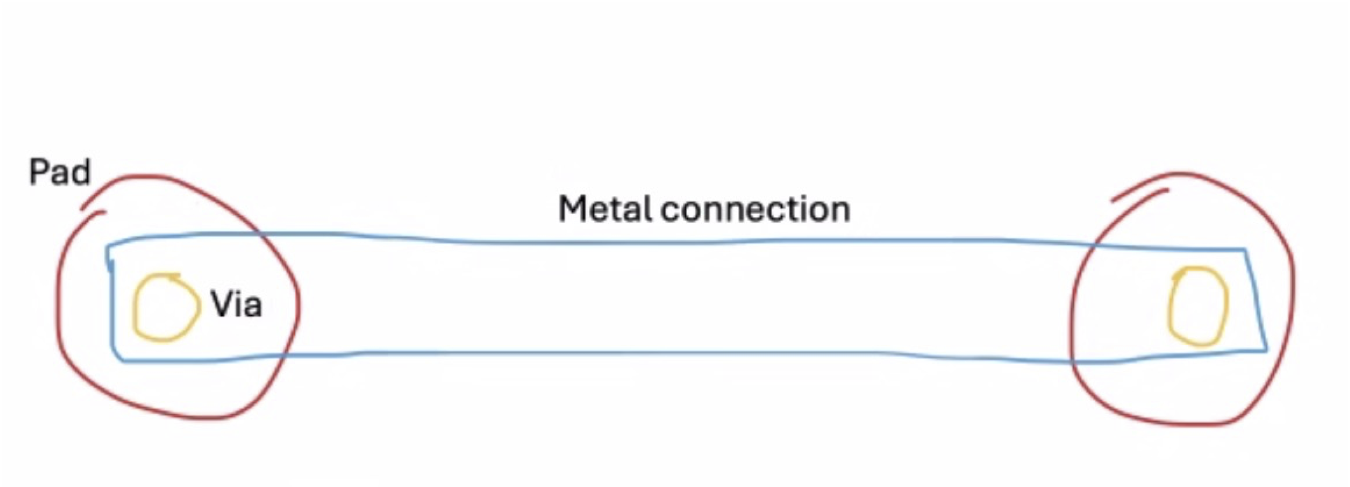
\includegraphics[width=0.5\linewidth]{sketch.png}

\textbf{Prompt for Test 2:} "I have a sketch idea that i want to draw in GDSII, generate the python code for this design. each color represents an individual layer. We want to have two vias near each end on a piece of metal. And a pad on top of the metal."; with graphical input of the sketch:
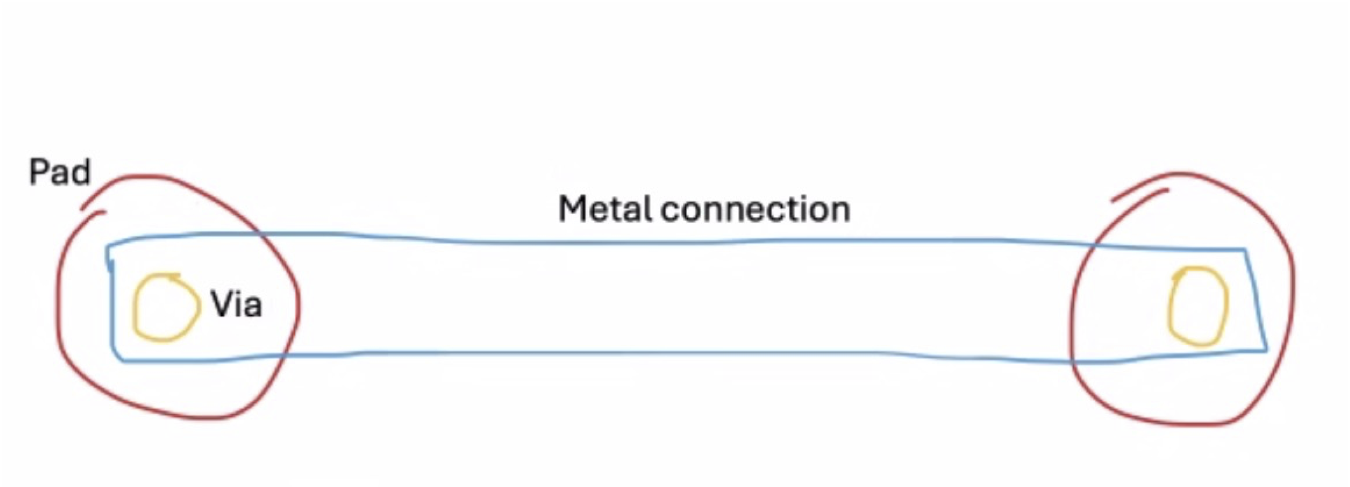
\includegraphics[width=0.5\linewidth]{sketch.png}

\textbf{Prompt for Test 3:} "I have a sketch idea that i want to draw in GDSII, generate the python code for this design. each color represents an individual layer. we want use to connect two vias using a piece of metal and put a circular padding on top of each via"; with graphical input of the sketch:
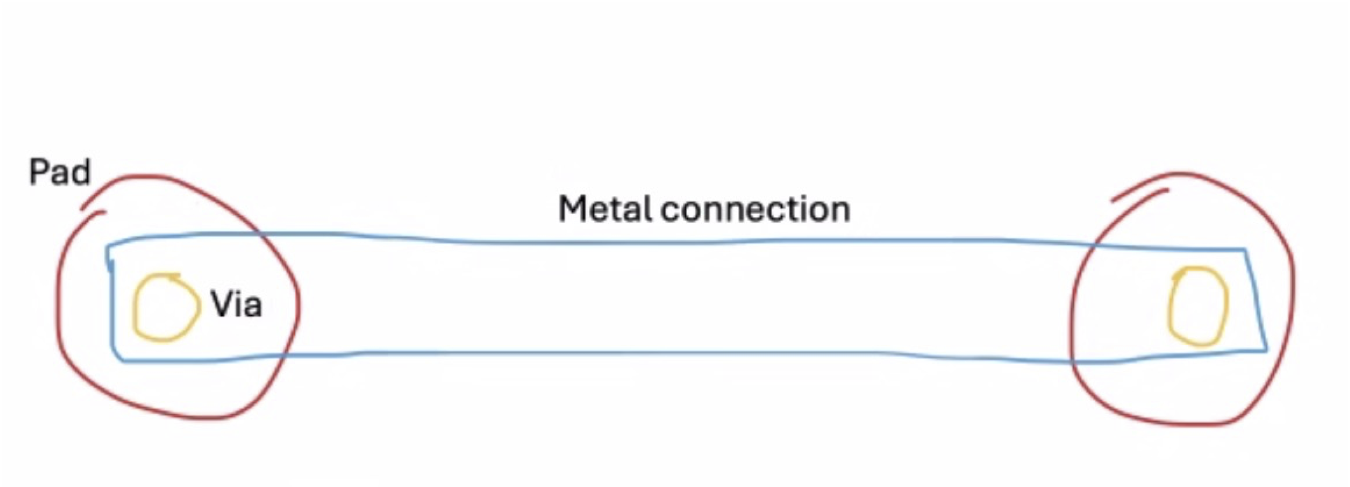
\includegraphics[width=0.5\linewidth]{sketch.png}


\begin{figure}[!th]
\centering
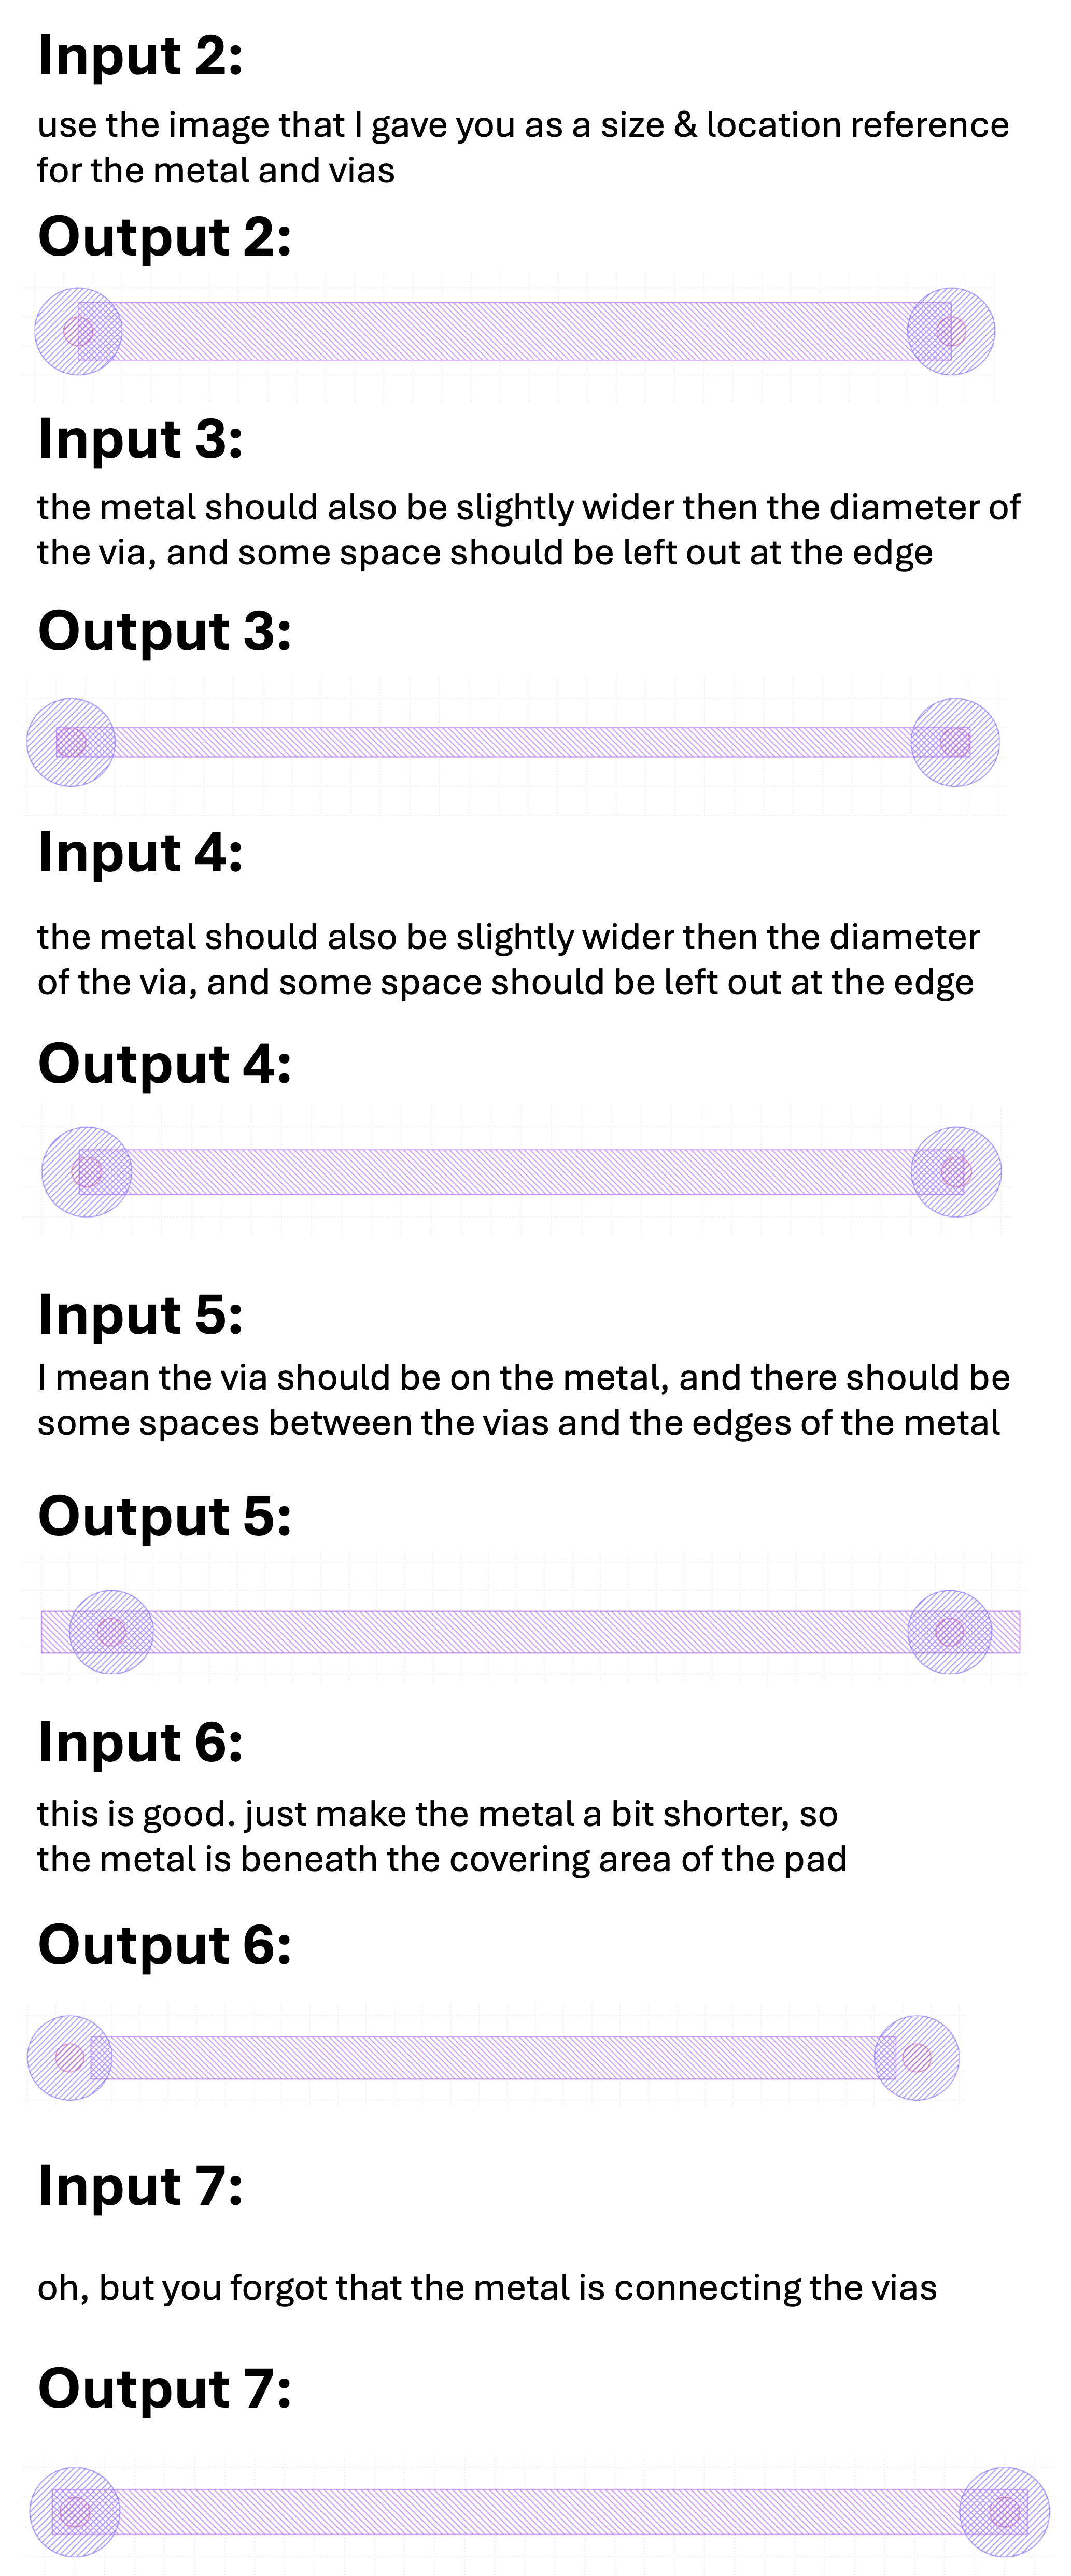
\includegraphics[width=0.5\linewidth]{Styles/Test3.png}
\caption{Iterations to guide the model to generate desired output}
\label{fig:test3}
\end{figure}

\textbf{Prompt for Test 4 (Generated by LLM based on the final output in Test 3):}\\
"Layers and Colors:
The design consists of three layers: via layer (yellow), metal layer (blue), and pad layer (red).\\
Dimensions:
Via: The radius of each via is 10 units.
Pad: The radius of each pad is 30 units.
Metal Connection: The width of the metal connection is 40 units, and the total length is 600 units.\\
Positions:
The first via is positioned at coordinates (50, 150).
The second via is positioned at coordinates (550, 150).\\
Connections and Coverage:
The metal connection should fully cover the vias, extending slightly beyond their edges.
Ensure the metal connection is slightly wider than the via diameter to provide full coverage.\\
Spacing and Margins:
Leave a margin of 10 units between the edge of the metal and the pads.
Ensure there is a space of 50 units between the vias and the edges of the metal connection.\\
Additional Requirements:
The metal connection should be shorter than the total length to fit beneath the covering area of the pads, leaving some space at the edges.
By providing detailed information like this, you can ensure that the design is accurately reproduced. If you have any specific design rules or preferences, make sure to include those as well."

\end{document}